\documentclass{article}%standalone can be used
\usepackage{tikz}
\usetikzlibrary{positioning}

\begin{document}
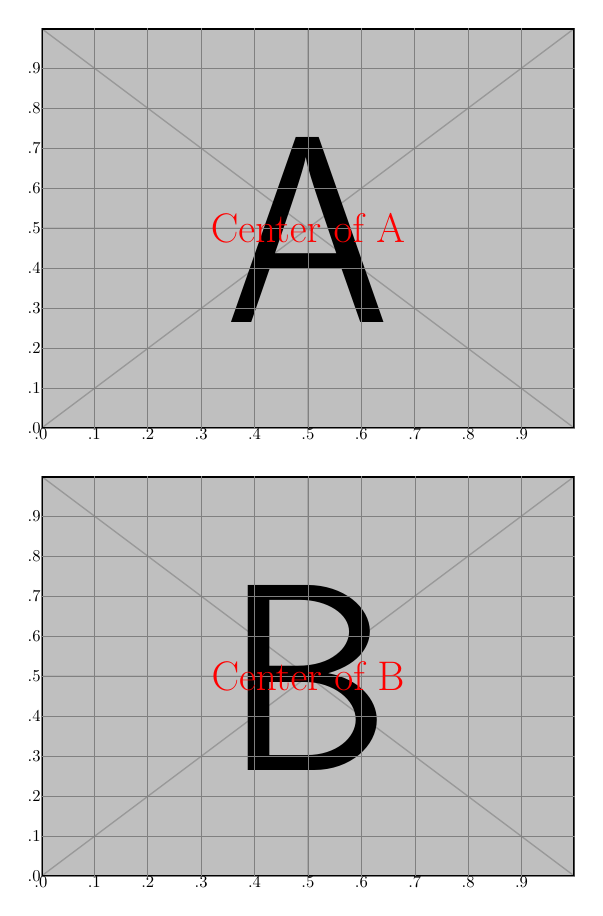
\begin{tikzpicture}[transform shape, scale=0.6, every node/.style={inner sep=0}]
    \node[anchor=south west] (image) {\includegraphics{example-image-a}};
    \begin{scope}[shift={(image.south west)},x={(image.south east)},y={(image.north west)}]
        \draw[help lines,xstep=.1,ystep=.1] (0,0) grid (1,1);
        \foreach \x in {0,1,...,9} {\node[anchor=north] at (\x/10,0) {.\x}; }
        \foreach \y in {0,1,...,9} {\node[anchor=east] at (0,\y/10) {.\y};}
        \begin{scope}[x={(image.south east)},y={(image.north west)}]
            % draw something on image a
            \draw (.5,.5) node[text=red, font=\Huge] {Center of A};
        \end{scope}
    \end{scope}

    \node (image) [below=of image] {\includegraphics{example-image-b}};
    \begin{scope}[shift={(image.south west)},x={(image.south east)},y={(image.north west)}]
        \draw[help lines,xstep=.1,ystep=.1] (0,0) grid (1,1);
        \foreach \x in {0,1,...,9} {\node[anchor=north] at (\x/10,0) {.\x}; }
        \foreach \y in {0,1,...,9} {\node[anchor=east] at (0,\y/10) {.\y};}
        \begin{scope}[x={(image.south east)},y={(image.north west)}]            
            % draw something on image b
            \draw (.5,.5) node[text=red, font=\Huge] {Center of B};
        \end{scope}
    \end{scope}
\end{tikzpicture}
\end{document}
